\subsection{CubeSat}\label{sec: CubeSat}

Der CubeSat, initiiert vom TU Wien Space Team, ist eine Bildungsmission, die im August 2020 gestartet wurde. Es handelt sich um einen CubeSat, der entwickelt wurde, um Schülern in Österreich die Möglichkeit zu bieten, eigene Software auf ihm auszuführen. Der Satellit enthält eine Bildungsnutzlast mit einem Raspberry Pi, Sensoren und Kameras, die von Schülern über Python programmiert werden können. Ziel ist es, durch den Betrieb dieses CubeSats und einer eigenen Bodenstation das Interesse und Wissen über Raumfahrttechnologien zu fördern.\\
\begin{figwindow}[0,r,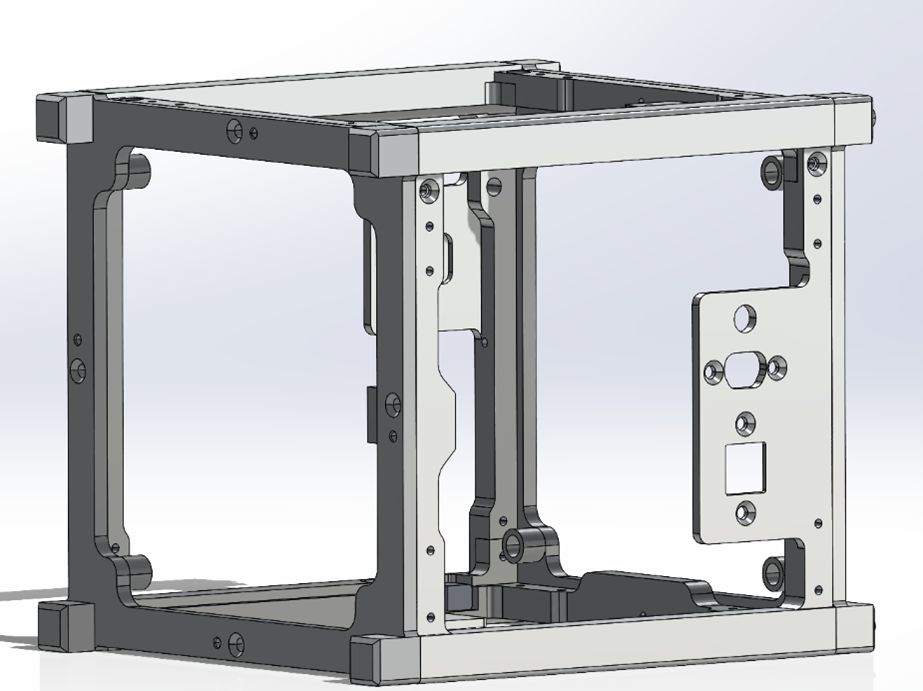
\includegraphics[scale=0.7]{image/3dcube.png},{3D-Modell des CubeSats}]
Das detaillierte Modell des CubeSats im Dateiformat für SolidWorks habe ich von der Technischen Universität Wien erhalten. Dieses hochpräzise Modell stellt eine wesentliche Ressource für die Diplomarbeit dar. Das bereitgestellte CubeSat-Modell zeichnet sich durch seine Detailgenauigkeit aus. 
\end{figwindow}
\vspace{25mm}
\begin{figure}[H]
    \centering
    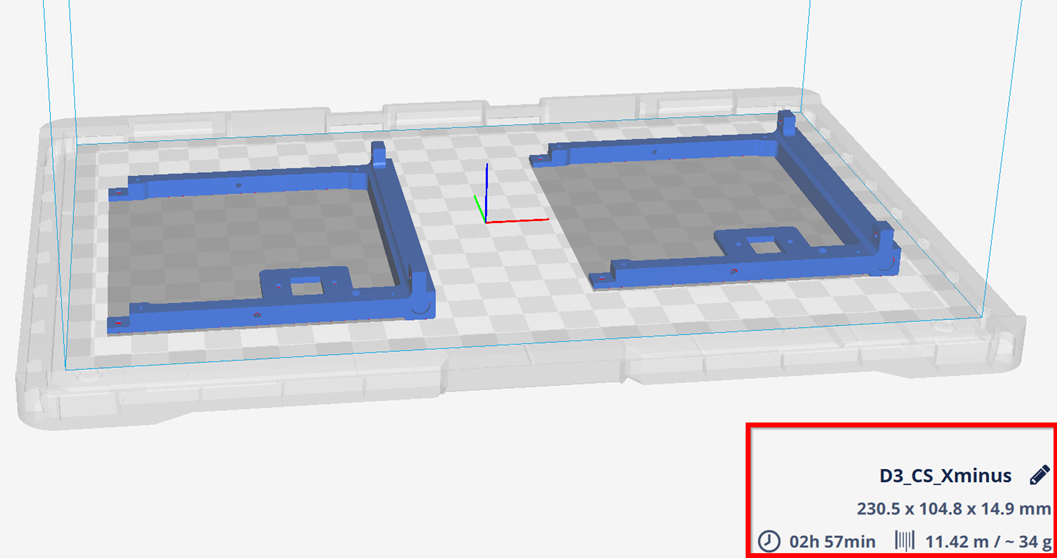
\includegraphics[scale = 0.8]{image/Druckvorbereitung.png}
    \caption{Druckvorbereitung von zwei Teilen des CubeSats}
    \label{fig:enter-label}
\end{figure}
\newpage
Wie man dem Bild entnehmen kann, sieht man auch, wie lange der Druckvorgang dauert, wie viele Meter Filament benötigt werden und wie viel der Druck wiegt.\\ 
Da sechs Seiten mit dem 3D-Drucker gedruckt werden müssen und maximal zwei Teile gleichzeitig gedruckt werden können, muss man den Vorgang mit den jeweiligen Teilen noch zweimal wiederholen. \\
\vspace{3mm}
\begin{figwindow}[0,r,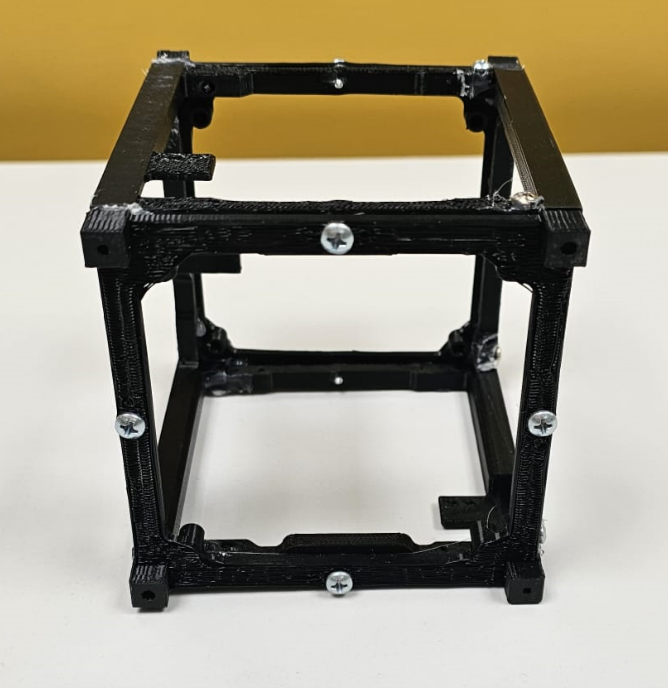
\includegraphics[scale=0.7]{image/ausdruck.png},{Ausgedrucktes Modell des CubeSats}]
Nachdem alle Teile des CubeSats gedruckt worden sind, muss der CubeSat noch zusammengeschraubt werden.  
\end{figwindow}
\vspace{55mm}
Um den Raspberry Pi sicher an einer Metallplatte zu befestigen, wurden vier Löcher in die Platte gebohrt. Für die Montage kamen spezielle Kunststoffschrauben, Standbolzen und Muttern zum Einsatz, um Kurzschlüsse zu vermeiden.\\
\vspace{3mm}
\begin{figure}[H]
    \centering
    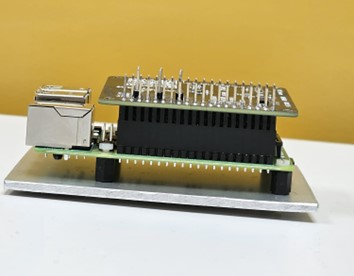
\includegraphics[scale = 0.7]{image/metalplatte.jpg}
    \caption{Raspberry Pi an der Metallplatte befestigt}
    \label{fig:enter-label}
\end{figure}
Der Raspberry PI wurde aufgrund von Stabilitätsgründen mit Abstandbolzen auf einer Metallplatte montiert und aus Isolationsgründen wurden Abstandsbolzen aus Kunststoff verwendet. Durch diese sorgfältige Vorgehensweise konnte ich sicherstellen, dass der Raspberry Pi optimal für seinen Einsatz im CubeSat vorbereitet ist, ohne die Sicherheit und Zuverlässigkeit des Systems zu gefährden.\\
\vspace{3mm}
\begin{table}[H]
    \centering
    \begin{tabular}{ | c | c | } 
  \hline
   \textbf{Bezeichnung} & \textbf{Stückzahl}\\ 
  \hline
   Kunststoffschrauben (M2,5) & 4\\ 
  \hline
  Kunststoffstandbolzen & 4 \\ 
  \hline
  Kunststoffmuttern & 4\\
  \hline
\end{tabular}
    \caption{Stückliste CubeSat}
\end{table}
Um eine optimale Haftung zu erzielen, wurde die Metallplatte mit dem Epoxidkleber sorgfältig am CubeSat angebracht. Bei diesem Vorgang kommt eine Schraubzwinge zum Einsatz, ein entscheidendes Werkzeug, um Druck auszuüben und so die Platte während des Aushärteprozesses des Klebers fest an ihrem Platz zu halten.\\
\vspace{3mm}
Die Schraubzwinge gewährleistet, dass der Kleber gleichmäßig verteilt wird und keine Luftblasen oder Unregelmäßigkeiten die Verbindung schwächen können. Diese Methode garantiert eine hohe Zuverlässigkeit, Stabilität und Halt für die späteren Rotationstests.\\
\vspace{3mm}
\begin{figure}[H]
    \centering
    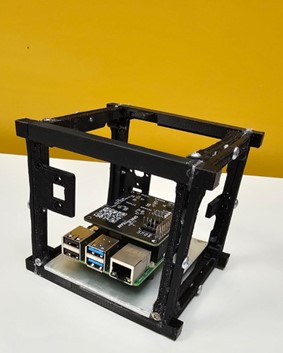
\includegraphics[scale = 0.7]{image/fertigercube.jpg}
    \caption{Fertiges CubeSat-Modell}
    \label{fig:enter-label}
\end{figure}
Abbildung zeigt den CubeSat mit der erfolgreich angepassten Aluminiumplatte mit dem Raspberry Pi.\\
